\documentclass{article}

\usepackage{graphicx}
\usepackage{tikz}
\usepackage{tikzsymbols}
\usetikzlibrary{calc,patterns,shapes.geometric}
\pagestyle{empty}
\usepackage[margin=0pt]{geometry}
\geometry{papersize={14in,12in}}

\def\centerarc[#1](#2)(#3:#4:#5){\draw[#1] ($(#2)+({#5*cos(#3)},{#5*sin(#3)})$) arc (#3:#4:#5);}

\begin{document}
	\begin{figure}
		\centering
		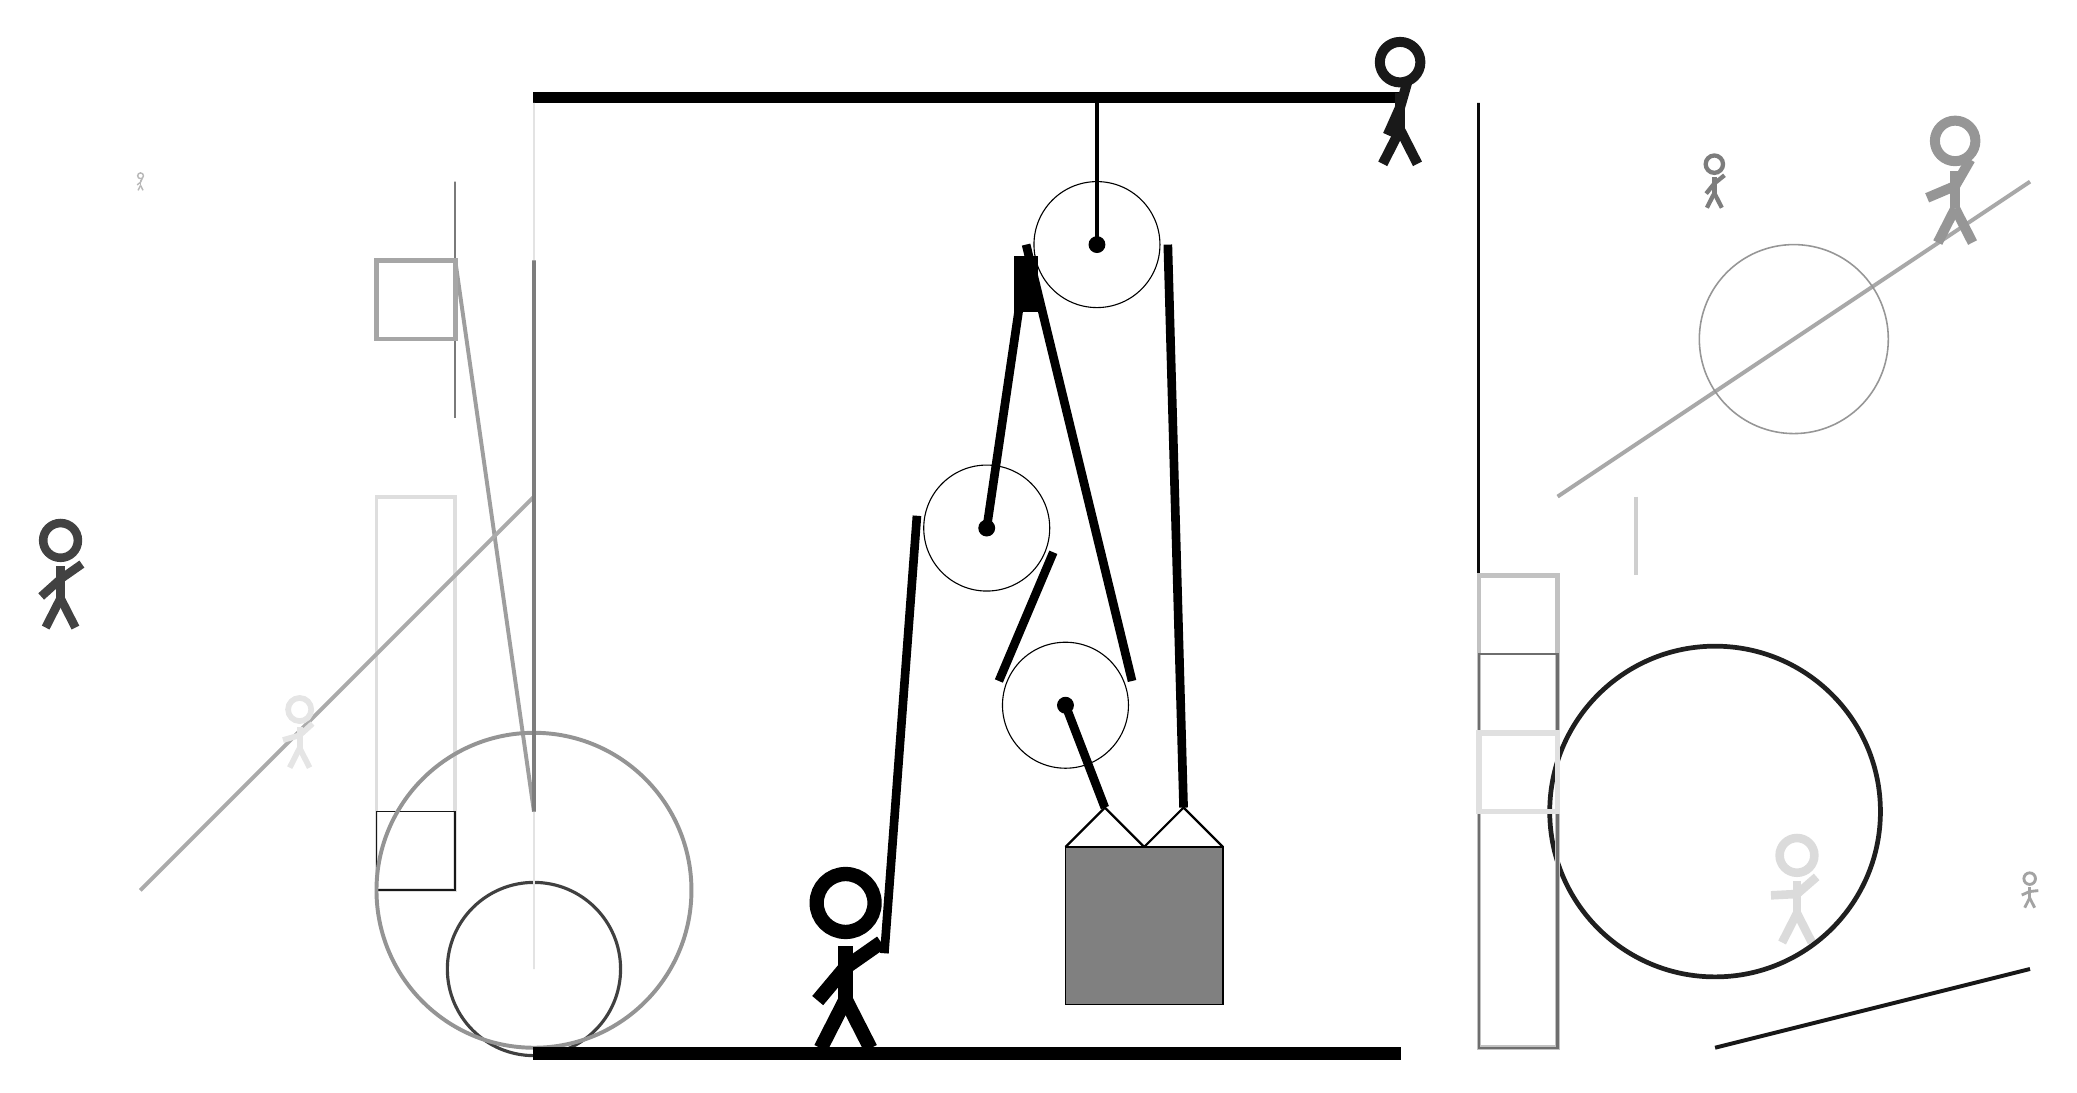
\begin{tikzpicture}
			%%%%% START %%%%%
			
			\draw[fill=black] (-6, 9) rectangle (5, 9.125);
			
			\draw (-0.25, 3.6) circle (0.8);
			\draw[fill=black] (-0.25, 3.6) circle (0.1);
			
			\draw (0.75, 1.35) circle (0.8);
			\draw[fill=black] (0.75, 1.35) circle (0.1);
			
			\draw (1.15, 7.2) circle (0.8);
			\draw[fill=black] (1.15, 7.2) circle (0.1);
			\draw[very thick] (1.15, 7.2) -- (1.15, 9);
			
			\draw [line width=0.4mm, color=black!75](-6, -2) circle (1.1);
			
			\draw[line width=0.4mm, color=black!80] (6, 3) rectangle (6, 3);
			\node[line width=0.5mm, color=black!14] at (10, -1) {\Strichmaxerl[6][3][41]};
			\draw[line width=0.2mm, color=black!52] (-7, 8) rectangle (-7, 5);
			\draw [line width=0.6mm, color=black!88](9, 0) circle (2.1);
			\draw[line width=0.4mm, color=black!96] (6, 0) rectangle (6, 9);
			
			\draw[line width=0.5mm, color=black!13] (-8, 4) rectangle (-7, -1);
			\draw[line width=0.2mm, color=black!91] (-7, -1) rectangle (-8, 0);
			\draw[line width=0.5mm, color=black!34](7, 4) -- (13, 8);
			\draw[line width=0.6mm, color=black!24] (7, 3) rectangle (6, -3);
			\draw[line width=0.5mm, color=black!38](-7, 7) -- (-6, 0);
			\node[line width=0.3mm, color=black!74] at (-12, 3) {\Strichmaxerl[6][42][35]};
			\draw[line width=0.5mm, color=black!91](9, -3) -- (13, -2);
			\draw[line width=0.5mm, color=black!19](8, 4) -- (8, 3);
			\node[line width=0.7mm, color=black!51] at (9, 8) {\Strichmaxerl[3][51][39]};
			\node[line width=0.3mm, color=black!90] at (5, 9) {\Strichmaxerl[7][66][74]};
			
			\draw [line width=0.2mm, color=black!41](10, 6) circle (1.2);
			\draw[line width=0.3mm, color=black!57] (6, -3) rectangle (7, 2);
			\node[line width=0.6mm, color=black!41] at (12, 8) {\Strichmaxerl[7][23][60]};
			
			\draw[line width=0.6mm, color=black!35] (-7, 7) rectangle (-8, 6);
			\node[line width=0.5mm, color=black!36] at (13, -1) {\Strichmaxerl[2][24][6]};
			
			\draw[line width=0.5mm, color=black!33](-11, -1) -- (-6, 4);
			\draw[line width=0.3mm, color=black!11] (-6, 9) rectangle (-6, -2);
			\draw [line width=0.5mm, color=black!42](-6, -1) circle (2.0);
			\draw[line width=0.5mm, color=black!51] (-6, 0) rectangle (-6, 7);
			\node[line width=0.5mm, color=black!10] at (-9, 1) {\Strichmaxerl[4][16][42]};
			
			\node[line width=0.4mm, color=black!28] at (-11, 8) {\Strichmaxerl[1][38][66]};
			\draw[line width=0.7mm, color=black!12] (6, 0) rectangle (7, 1);
			
			\draw[thick]  (0.75, -0.45) -- (1.25, 0.05) -- (1.75, -0.45) -- (2.25, 0.05) -- (2.75, -0.45);
			\draw[fill=black!50] (0.75, -0.45) rectangle (2.75, -2.45);
			
			\draw[line width=1.1mm] (-0.25, 3.6) -- (0.25, 7.0);
			\draw[line width=1.1mm, fill=black](0.15, 6.4) rectangle (0.35, 7.0);
			\draw[line width=1.1mm] (-1.55, -1.8) -- (-1.1363, 3.7562);
			\centerarc[line width=1.1mm](-0.25, 3.6)(-20:170:0.9);
			\draw[line width=1.1mm] (0.5957, 3.2922) -- (-0.0957, 1.6578);
			\centerarc[line width=1.1mm](0.75, 1.35)(160:380:0.9);
			\draw[line width=1.1mm] (1.5957, 1.6578) -- (0.25, 7.2);
			\draw[line width=1.1mm](0.75, 1.35) -- (1.25, 0.05);
			\centerarc[line width=1.1mm](1.15, 7.2)(0:180:0.9);
			\draw[line width=1.1mm] (2.05, 7.2) -- (2.25, 0.05);
			
			\node at (-2, -1.9) {\Strichmaxerl[10][50][35]};
			
			\draw[fill=black] (-6, -3) rectangle (5, -3.15);
			
			%%%%% END %%%%%
		\end{tikzpicture}
	\end{figure}	
\end{document}